\capitulo{Procedimentos metodológicos e técnicos}
\label{cap:procedimentos-metodologicos-tecnicos}

Neste capítulo do trabalho será abordada a caracterização da metodologia de pesquisa, questões de pesquisa,
como será a aplicação da metodologia e o desenvolvimento do sistema computacional, além de mostrar como será a analise de resultados e a população e amostra do trabalho.

\secao{Caracterização da metodologia de pesquisa}
\label{sec:caracterizacao-metodologia-pesquisa}
    
O presente trabalho se caracteriza como uma metodologia aplicada, tendo uma abordagem quantitativa, buscando atingir seus objetivos de forma descritiva e exploratória através de procedimentos exploratórios e de um estudo de caso.

Segundo Gerhardt e Silveira (2009, p. 35), a pesquisa aplicada visa gerar conhecimentos para aplicação prática, dirigidos à solução de problemas específicos, buscando responder às necessidades concretas de organizações, instituições ou grupos sociais. 
Em complemento, Fonseca (2002) destaca que a pesquisa aplicada está orientada para transformar a realidade de forma direta, aplicando conhecimentos científicos já estabelecidos.

No que se refere à abordagem quantitativa, Gerhardt e Silveira (2009, p. 33) afirmam que esta traduz em números as informações e opiniões, classificando-as e analisando-as de forma objetiva, buscando generalizações estatísticas. Por explorar dados numéricos como a angulação e rotatividade do braço no movimento do arremesso, esse trabalho se caracteriza como quantitativo em sua abordagem.

A pesquisa exploratória, de acordo com Gil (2008, p. 27), tem como finalidade proporcionar maior familiaridade com o problema, visando torná-lo mais explícito ou construir hipóteses, sendo especialmente útil quando o fenômeno é pouco conhecido. 
Já a pesquisa descritiva, conforme Gil (2008, p. 28), objetiva descrever as características de determinada população ou fenômeno, bem como estabelecer relações entre variáveis. Esse trabalho se caracteriza como exploratório e descritivo, pois o mesmo interpreta dados biomecânicos para executar o estudo, além de abordar um ramo que hoje está em desenvolvimento no Brasil que é a Análise de Desempenho Esportiva.

No que tange aos procedimentos, Gerhardt e Silveira (2009, p. 36) indicam que a pesquisa experimental é caracterizada pela manipulação de variáveis para observar os efeitos provocados, sendo amplamente empregada em estudos controlados. A manipulação de variáveis dentro de um arremesso fazem com que este trabalho se caracterize como uma pesquisa experimental.
O estudo de caso, por sua vez, segundo Gil (2008, p. 57), busca uma análise profunda e exaustiva de um ou poucos objetos, proporcionando um conhecimento abrangente e detalhado da realidade investigada. O fator determinante para este trabalho ser um estudo de caso, se dá pelo fato de ser executado em uma equipe específica, sendo estudado de início somente com esse número pequeno de jogadores, para caso haja êxito, ser posteriormente evoluído a um estudo para outras equipes também.


    %Os procedimentos técnicos adotados neste trabalho envolvem a realização de uma \textbf{pesquisa experimental}, de um \textbf{estudo de caso} e de uma \textbf{pesquisa bibliográfica}.
    
    %A pesquisa experimental será conduzida mediante a captura de vídeos de arremessos realizados por atletas amadores, que serão analisados através de um modelo de visão computacional baseado em inteligência artificial. O objetivo é extrair variáveis biomecânicas, como ângulos articulares e trajetória da bola, permitindo a avaliação automatizada da técnica do arremesso.
    
    %O estudo de caso consiste na aplicação do modelo desenvolvido em um grupo específico de atletas, permitindo uma análise aprofundada de seus gestos técnicos e comparações com parâmetros ideais descritos na literatura. O enfoque será direcionado para um time amador que compete regionalmente, o que delimita o escopo da pesquisa.
    
    %A pesquisa bibliográfica complementa o estudo, fornecendo o embasamento teórico necessário para a definição dos padrões biomecânicos de referência, essenciais para a comparação e avaliação dos resultados obtidos.
    
    
\secao{Questões de Pesquisa}
\label{sec:questoes-pesquisa}

O protótipo proposto é capaz de capturar, processar e analisar biomecanicamente, 
com base em visão computacional, os movimentos do arremesso no basquetebol, 
fornecendo diagnósticos para auxiliar atletas e treinadores na correção do gesto de arremesso?

\secao{Aplicação da metodologia}
\label{sec:aplicacao-metodologia}

Nesta subseção, são descritas as etapas adotadas para o desenvolvimento da metodologia deste trabalho. As atividades englobam desde a preparação do ambiente de desenvolvimento e coleta de dados até a 
implementação dos algoritmos de visão computacional e a validação dos resultados obtidos. Cada fase foi conduzida com o objetivo de garantir a confiabilidade do sistema final e a coerência com os objetivos traçados neste trabalho.

\subsecao{Desenvolvimento da solução proposta na prática}
\label{ssec:populacao-amostra-participantes-estudo}

O modelo em cascata é uma das abordagens clássicas para o desenvolvimento de software e foi originalmente descrito por Winston Royce em 1970. 
Este modelo foi posteriormente estruturado por Ian Sommerville em sua obra clássica “Engenharia de Software” como um processo sequencial em que cada fase depende da entrega da anterior e gera um produto definido.

\begin{figura}{Modelo Cascata}{Sommerville (2011)}
    \begin{flushleft}
        \label{fig:modelo-cascata}
        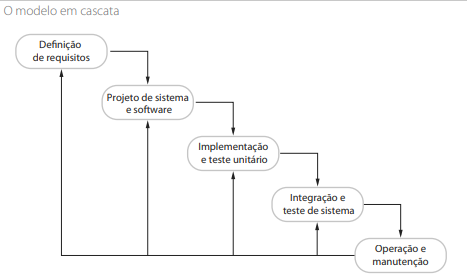
\includegraphics[width=0.95\linewidth]{resources/floats/ilustracoes/cascata.png}
    \end{flushleft}
\end{figura}

Conforme ilustrado na Figura 13 (Modelo cascata de Sommerville), o modelo é dividido em cinco fases principais: definição de requisitos, 
projeto de sistema e software, implementação e teste unitário, integração e teste de sistema, e operação e manutenção. 
Cada fase possui entregáveis específicos e critérios de entrada e saída bem definidos.

\subsubsecao{Definição de Requisitos}
\label{sssec:def-requisitos}

A definição de requisitos é a etapa de desenvolvimento de software que descreve detalhadamente o que o sistema deve fazer e quais restrições ele deve obedecer. 
De acordo com Sommerville (2011), um requisito é “uma descrição de algo que o sistema deve fazer ou uma propriedade que ele deve ter”. 
Essa definição engloba tanto funcionalidades esperadas quanto limitações técnicas ou organizacionais que devem ser consideradas na construção do projeto.

Ainda segundo Sommerville (2011), os requisitos funcionais especificam os serviços que o sistema deve oferecer e como ele deve reagir a entradas específicas. 
Por outro lado, os requisitos não funcionais dizem respeito a restrições sobre os serviços ou funções oferecidas, como requisitos de desempenho, padrões de qualidade, requisitos organizacionais ou de segurança. 
Para a obtenção desses requisitos, será adotada a técnica de entrevistas semiestruturadas com os usuários finais que serão de inicio os atletas participandes do estudo de caso. 
Essa abordagem permitirá captar informações sobre as necessidades práticas dos usuários, possibilitando uma definição mais precisa e contextualizada dos requisitos do sistema.

\subsubsecao{Projeto de Sistema e Software}
\label{sssec:proj-sistema}

\subsubsecao{Fase de Implementação}
\label{sssec:implementação}

\subsubsecao{Fase de integração e testes}
\label{sssec:testes}

A fase de testes é responsável por garantir a qualidade do software e a conformidade com os requisitos especificados. 
Segundo Pressman (2011), os testes de software devem ser planejados de forma sistemática e aplicados com o propósito de revelar o maior número possível de defeitos, contribuindo para a qualidade e confiabilidade do produto final.

Os testes serão divididos entre a verificação funcional da aplicação desenvolvida em Python e a avaliação do desempenho do modelo de detecção de imagens. 
O roteiro de testes considera a execução da aplicação com vídeos reais, gravados durante os treinos, que serão analisados quadro a quadro pelo modelo treinado. 
O objetivo é validar se as detecções ocorrem corretamente, se os dados gerados estão de acordo com os critérios esperados e se a experiência de uso da aplicação permanece fluida. 
As verificações funcionais incluem a leitura adequada dos arquivos de vídeo, a ativação correta do modelo, a identificação precisa de elementos como a bola de basquete e os membros superiores, 
além da geração de análises coerentes dos arremessos e do bom desempenho geral do sistema. Parte dos testes será também automatizada com o uso do framework PyTest, 
focando em funções auxiliares como o pré-processamento das imagens e a validação da integração com arquivos simulados, o que permite assegurar a estabilidade do sistema mesmo após possíveis futuras alterações no código.

\subsubsecao{Operação e manutenção}
\label{sssec:operação}

A fase de operação e manutenção corresponde à última etapa do ciclo de vida no modelo em cascata, sendo responsável por garantir a continuidade do funcionamento do sistema após sua entrega, 
além de contemplar ajustes, correções de falhas e melhorias que possam surgir com o uso contínuo da aplicação. De acordo com Pressman (2016), esta etapa não apenas envolve a correção de erros não detectados anteriormente, 
mas também a adaptação do software às mudanças de ambiente e requisitos, bem como o aprimoramento de sua funcionalidade.

Neste trabalho, serão feitas manutenções para o bom funcionamento do sistema, buscando sempre atualizações que melhorem a eficiência do mesmo. 
Possivelmente melhorias como a implementação de análises de outros movimentos, como passes ou bloqueios poderão ser feitas com manutenções posteriores a entrega do projeto inicial.

\subsecao{População e Amostra}
\label{sec:esboco-projeto-pratica}

A população desse estudo é composta por uma equipe de basquete, hoje competindo em âmbito amador, tendo um foco maior na modalidade de basquete 3x3. Atualmente a equipe conta com aproximadamente 15 atletas, onde serão selecionados alguns para a realização dos
testes deste trabalho.

A seleção não considerará variáveis como idade, posição em quadra ou nível técnico individual, visto que o objetivo da pesquisa é avaliar a aplicabilidade da ferramenta em um contexto coletivo e real de treinamento.






